%*******************************************************************************
%*********************************** First Chapter *****************************
%*******************************************************************************

\ifpdf
    \graphicspath{{Chapter1/Figs/Raster/}{Chapter1/Figs/PDF/}{Chapter1/Figs/}}
\else
    \graphicspath{{Chapter1/Figs/Vector/}{Chapter1/Figs/}}
\fi

\chapter{Introduction to Reactor Monitoring} \label{Chap:theAimOfVidarr} %Title of the First Chapter
% This chapter will go over the basic principle of anti-neutrino ($\bar{\nu}$) monitoring and what results are expected from this specific form of monitoring. There will be a light focus on what spectrum of energies will be expected from an $\bar{\nu}$ detector. But this chapter will mainly focus on the results and technology of other experiments currently in the field. This is done to give a grounded realistic view of what can be achieved with particular technology and setups. 
This chapter will go over the basic principles of reactor monitoring and measurement of reactor anti-neutrinos ($\bar{\nu}$) and will review detectors built for this purpose. The $\bar{\nu}$ detectors built at Liverpool, RMon and VIDARR, will be introduced in this chapter. The thesis as a whole will focus on the modelling of the VIDARR detector for future deployments and data analysis of cosmic $\mu$ data from RMon to illustrate the detector's performance in tomography.

\section{Reactor Anti-Neutrinos} \label{sec:reactorAntiNeutrinos}
Nuclear reactors produce high quantities of $\bar{\nu}$s, with on average 6 $\bar{\nu}$s emitted by the decay of fission products from each fission \cite{Mueller_2011}. $\bar{\nu}$s are prevalent over neutrinos as the fission products are overwhelmingly neutron rich and decay by $\beta^-$ emission towards stability. A typical nuclear reactor emits $\sim$ 10$^{20}$ $\bar{\nu}$s per GW$_{\textrm{Th}}$ \cite{Mueller_2011} and although only $\sim$3\,\% are above detection thresholds \cite{Mueller_2011}, the intensity of the detectable flux of $\bar{\nu}$ is still high enough for measurement. The first direct measurement of $\bar{\nu}$s was achieved in 1953 by Cowan and Reins using $\bar{\nu}$s from a nuclear reactor \cite{reines1953detection}. The response of $\bar{\nu}$s was measured in cadmium-doped liquid scintillator \cite{reines1953proposed} \cite{Cowan1956Confirmation} via the inverse $\beta$ decay (IBD) process. At the Hanford site Cowan and Reins measured a difference due to the pile of $0.41 \pm 0.20$ delayed count/min\cite{reines1953detection}, measuring what was most likely a 250\,MW$_{\textrm{th}}$ reactor, though the stand off does not appear to have been recorded. This was the first time reactor monitoring had been achieved via the use of $\bar{\nu}$ measurements. 
%ADD X events were measured in Y time in a Z tonne detector, @ metres from the £ GWTe &&& reactor.

\subsection{Inverse Beta Decay} \label{subSec:IBD}
%The Cowan and Reins and subsequent measurements of reactor $\bar{\nu}$s used 
Subsequent measurements of reactor $\bar{\nu}$s by Cowan, Reins, and others used
the IBD reaction of 1H atoms in their target material \cite{Cowan1956Confirmation} \cite{sno2001} \cite{superK2001}. In the IBD reaction (equation \ref{inverse_beta_decay}, and figure \ref{fig:inverse_beta_diagram}), the $\bar{\nu}$ is absorbed by the proton giving a neutron and positron in  it's final state. This reaction proceeds only via the weak interaction which doesn't conserve flavour as inverse $\beta$ decay seen in figure \ref{fig:inverse_beta_diagram} relies on an up quark transitioning to a down quark (uud (proton) $\rightarrow$ udd (neutron)). And as a consequence has a extremely small cross-section of O(10$^{-42}$) cm$^2$\cite{Vogel_1999}. This also provides the ability for neutrinos to be observed even with significant shielding around the source. With the large mass difference between the positron and neutron, the majority of energy is carried away by the positron with the neutron only having O(10\,keV) of kinetic energy \cite{Vogel_1999}.

%The VIDARR detector observes $\bar{\nu_e}$s via inverse $\beta$ decay  via the weak interaction. The weak interaction doesn't conserve flavour as inverse $\beta$ decay seen in figure \ref{fig:inverse_beta_diagram} relies on an up quark transitioning to a down quark (uud $\rightarrow$ udd), this process can only be enabled through the weak interaction. This process is mediated through the W boson, not the, Z as the interaction has charged particles and charge must still be conserved in weak interactions. Neutrinos only interact with other matter through the weak interaction. This leads to a small cross section of 10$^{-42}$\,cm$^2$\cite{Vogel_1999}, making $\bar{\nu}$s difficult to detect. This also provides the ability for neutrinos to be observed even with significant shielding around the source. 
\begin{equation}
    \Bar{\nu_e} + p^+ \rightarrow n + e^+
    \label{inverse_beta_decay}
\end{equation}

\begin{figure}[!h]
  \centering
  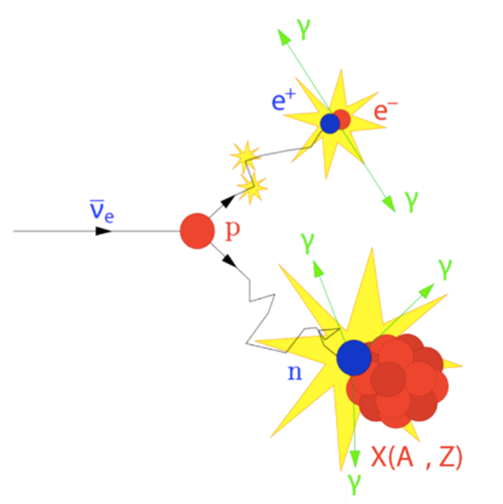
\includegraphics[width=0.5\linewidth]{Chapter2/Figs/Raster/inverse_beta_diagram.png} 
  \captionof{figure}{A diagram of inverse $\beta$ decay 
 (equation \ref{inverse_beta_decay}). The neutrons random walk means it will take (O $\sim$ 10 $\mu$s) before it is detected but the positron emission is prompt. From \cite{ibdPictureLink}.}
  \label{fig:inverse_beta_diagram}
\end{figure}

In a reactor $\sim$ 200\,MeV is released per fission and $\sim$ 6 neutrinos along the $\beta$ decay chain are produced \cite{Mueller_2011}. ``Since unstable fission products are neutron-rich nuclei all $\beta$ decays are of $\beta^-$ type and the neutrino flux is actually pure electronic $\bar{\nu}$s ($\bar{\nu_e}$)''\cite{Mueller_2011}, meaning that the $\bar{\nu_e}$s are the main particles of interest for reactor studies. Neglecting the small kinetic energy of the neutron, the kinetic energy of the positron may be related to the $\bar{\nu}$ via equation \ref{nu_energy_eq} which shows the $\bar{\nu_e}$ energy in terms of well known quantities, the kinetic energy and rest mass of the $e^+$ and the masses of the neutron and proton \cite{Vogel_1999}. 
\begin{equation}
 E_{\bar{\nu_e}} = T_{e^+} + m_{e}c^2 + (m_n - m_p)c^2  %E_{e^+} + (M_n - M_p) 
\label{nu_energy_eq}
\end{equation}

\section{Anti-Neutrino Reactor Monitoring}
% Obviously the two papers to mention here are vogal and beacom 1999 \cite{Vogel_1999} and muller et al 2011 \cite{Mueller_2011}. They cover the ground pretty well. \cite{Mueller_2011} has the $10^{20}$ $\Bar{\nu_e}$/s per GW$^{Th}$ and \cite{Vogel_1999} has the cross section values. \cite{Vogel_1999} is mostly dealing with stuff to first order, it may be worth addressing how this changes with increasing order. But probably not considering the low number of events $\bar{\nu}$ detection yields. Worth also going over the cowan and riens \cite{Cowan1956Confirmation} \cite{cowan1957test} again just briefly. The songs s1 project is also a necessity in 2007 it marked the beginning of serious reactor monitoring \cite{Bowden_2007}. And of course the original soviet paper which suggested this is as a possibility \cite{Borovoi_1978}. Also need to mention the IAEA and there workshop which suggested the limitations for this \cite{IAEA_2008}. 
% \\\\Probably best to go onto semi chronologically with the Cowan and Reins approach stating that reactor monitoring was one of the original approaches as fuel decays through beta decay (equation \ref{modern_beta_decay}) and the detection occurs through equation \ref{inverse_beta_decay}. It may be worth also mentioning section \ref{Direct_Measurements_section}. Then mentioning the soviet paper \cite{Borovoi_1978} then the move on to the first prototype with SONGS1 and then \cite{Bowden_2007} which then informed the IAEA report \cite{IAEA_2008}. Then talk about vogel \cite{Vogel_1999} and muller \cite{Mueller_2011}.
In 1978 it was proposed that measuring $\bar{\nu}$s from reactors could be used for reactor monitoring \cite{Borovoi_1978}. However, due to the geopolitics of the time, the interest in non-proliferation was not as high as in modern times. It took until 2007 for the SONGS1 prototype to be deployed as proof of concept for reactor monitoring \cite{Bowden_2007}.
%Reactor monitoring was used to prove the existence of neutrinos. In 1953 the direct measurements of $\bar{\nu_e}$ from reactors was done by Cowan and Reins \cite{Cowan1956Confirmation}. The response of $\bar{\nu}$s was measured in cadmium-doped liquid scintillator \cite{Cowan1956Confirmation} which used inverse $\beta$ decay (equation \ref{inverse_beta_decay}). This will be expanded upon in section \ref{Direct_Measurements_section}. $\sim$ 20 years after that experiment %in 1978 it was proposed that measuring $\bar{\nu}$s from reactors could be used for reactor monitoring \cite{Borovoi_1978}. However, due to the geopolitics of the time, the interest in non-proliferation was not as high as in modern times. It took until 2007 for the SONGS1 prototype to be deployed as proof of concept for reactor monitoring \cite{Bowden_2007}. 
\\\\After the deployment of the SONGS1 prototype the International Atomic Energy Agency (IAEA) workshopped a list of positive traits that they would like to see in an $\bar{\nu}$ reactor monitoring detector. These traits include inert construction, non-liquid, easy operation, cheap, portable, robust, above-ground operation, and easy deployment \cite{IAEA_2008}. Whilst these are not requirements, all of these traits can be met in a single detector. For example, VIDARR and RMon meet all of these traits, as they were purpose built to do so. 
\\\\For reactors that operate for long periods without refuelling, $\bar{\nu}$ monitoring has the potential to correlate the measured spectra with build up of $^{239}$Pu in the core, and determine when and how often refuelling occurs. This information is useful for non-proliferation purposes. However, this is not possible for reactors that may refuel online such as Advanced Gas-Cooled Reactors (AGRs) and pebble bed reactors. Though for these, the potential to monitor composition is interesting (although this would require spectral measurements).
% \\\\Reactors produce O $\sim$ $10^{20}$ $\Bar{\nu_e}$/s per GW$^{Th}$ as the fission products in the fuel elements $\beta$ decay \cite{Mueller_2011}. Though these rates are very high, the interaction cross-section to first order is $\sim 10^{-42}$cm$^2$ as can be seen in figure \ref{mullerAndVogelCombined} \cite{Vogel_1999}. In addition to this different fission, fractions will decay at different rates as can be seen in figure \ref{mullerAndVogelCombined}. The combination of these two effects can be seen in figure \ref{fig:anSpectraIsotopes} \cite{Mueller_2011}. From figure \ref{fig:anSpectraIsotopes} the range of $\bar{\nu}$ energies expected to be detected ranges from $\sim$ 1.8\,MeV to $\sim$ 8.5\,MeV. The threshold is 1.804\,MeV as this is the mass difference between the initial and final states \cite{Mueller_2011}. The true threshold energy of the reaction is slightly higher 1.806\,MeV, as the relativistic neutrino momentum requires the neutron and $e^+$ to have some momenta \cite{Vogel_1999}. Immediately after an IBD, the positron will annihilate giving two 511\,keV $\gamma$-rays and the neutron will thermalise in the detector medium before capture. The time taken for thermalisation causes a characteristic double coincidence signal with a delay between a prompt signal from positron interactions and the later neutron capture. This double coincidence may be used to select IBD events from background events. Dependent on the detector media, the mean time between positron and neutron signals is 10\,$\mu$s -- 100\,$\mu$s.

% \begin{table*}[!h]
% \centering
% \begin{tabular}{ll}  
% %\toprule
% %\midrule
% 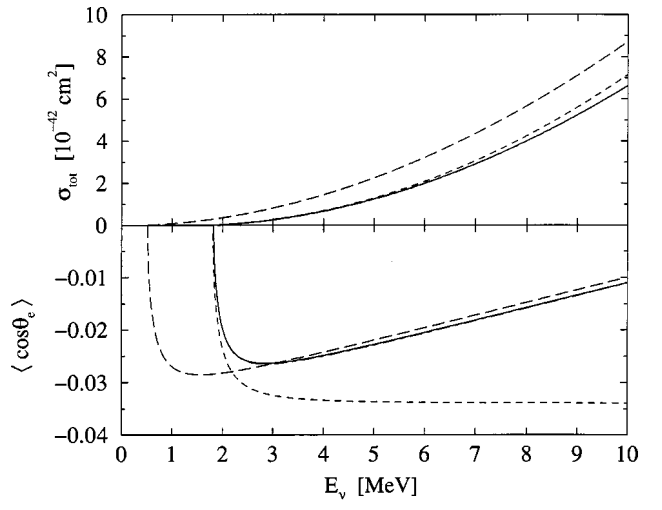
\includegraphics[width=0.49\linewidth]{Chapter1/Figs/Raster/vogelAndBeacomCrossSection.png} &    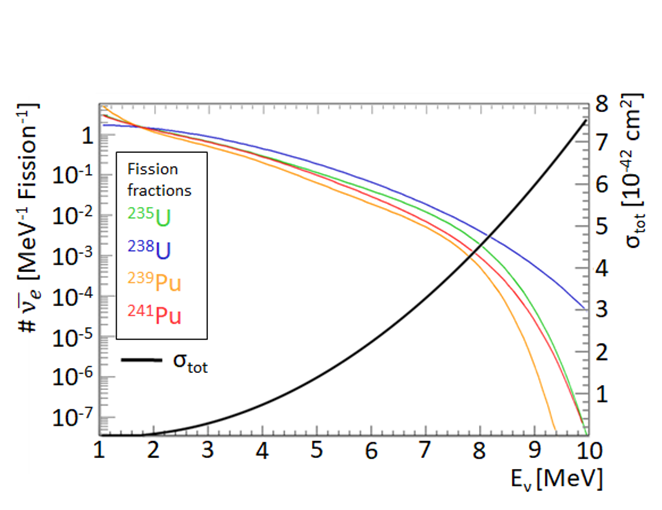
\includegraphics[width=0.49\linewidth]{Chapter1/Figs/Raster/mullerAndVogelCombined.png}\\
%  Upper panel: total cross-section for Inverse $\beta$ decay; bottom panel: $\bra{}\cos(\theta)\ket{}$ for the same reaction; both as a function of the $\bar{\nu}$ energy. The solid line is the O(1/M) result and the short-dashed line is the O(1) result. The long-dashed line is the result of Eq. 3.18. From \cite{smith_1972} \cite{Vogel_1999}. a & fig b\\
% %\bottomrule  
% \end{tabular}
% %\caption{a table figure test}
% \label{tab:figTest}
% \end{table*}

\begin{figure}[!h]
\centering
\begin{minipage}{.45\textwidth}
  \centering 
  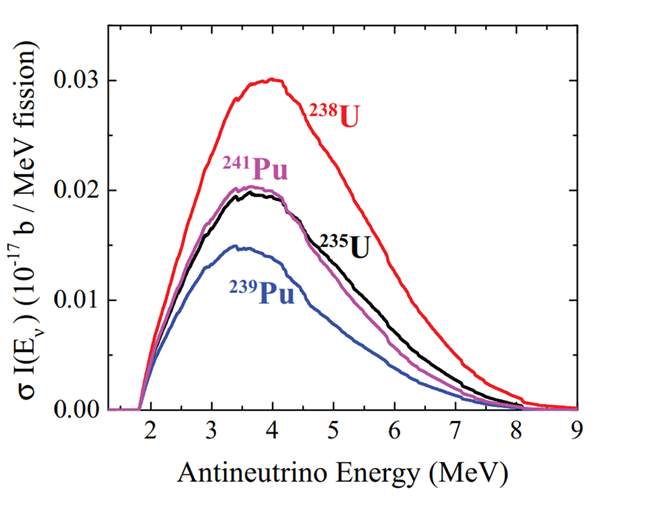
\includegraphics[width=\linewidth]{Chapter1/Figs/Raster/detectedNueSpectrumMultipleIsotopes.png}
  \captionof{figure}{$\bar{\nu}$ spectra multiplied by the $\bar{\nu} + p \rightarrow n + e^+$ cross section for the thermal fission of $^{235}$U and $^{239,241}$Pu and the fast fission of $^{238}$U. From \cite{sonzogni_nucStrcutre_2015}.} 
  \vspace{0.478cm} %1 line = 0.478cm % 2 lines = 0.956cm % 3 lines= 1.434cm % 4 lines = 1.912cm % 5 lines = 2.39cm
  \label{fig:anSpectraIsotopes}
  \end{minipage}
  \qquad
\begin{minipage}{.45\textwidth}
  \centering
  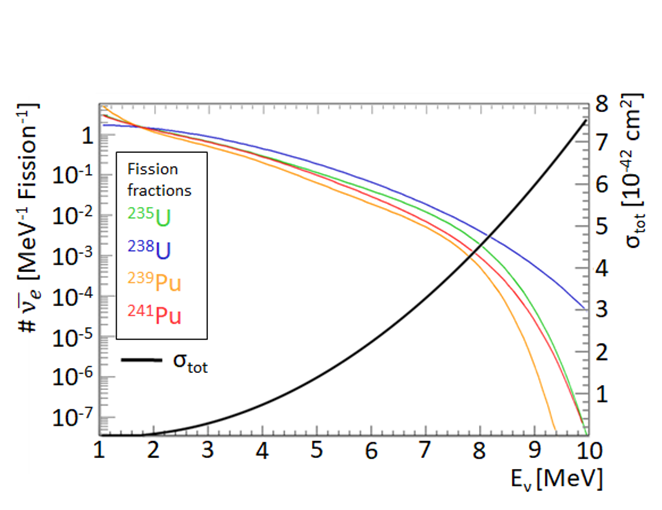
\includegraphics[width=\linewidth]{Chapter1/Figs/Raster/mullerAndVogelCombined.png} 
  \captionof{figure}{A combination of the fission fractions from \cite{Mueller_2011} and the first-order approximation of the cross-section from \cite{Vogel_1999} and their evolution over the energy range where the two distributions cross over.}
  \label{mullerAndVogelCombined}
\end{minipage}%
\end{figure}

% \begin{figure}[!h]
%  \centering
%  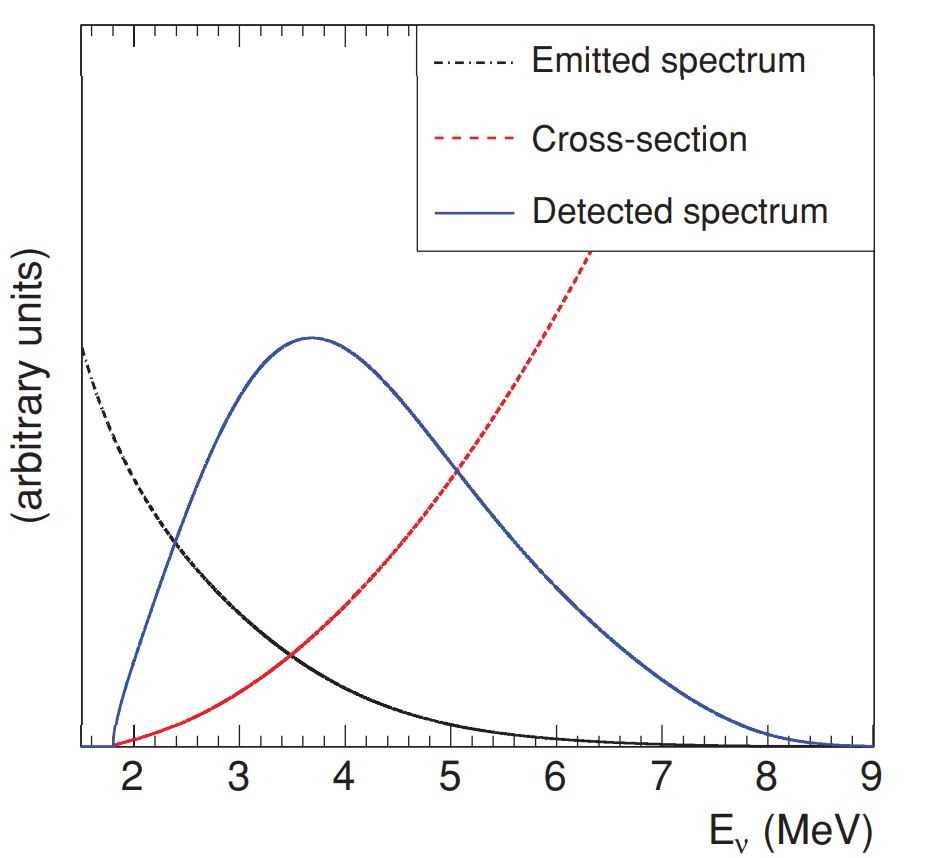
\includegraphics[width=0.4\linewidth]{Chapter1/Figs/Raster/mullerEtAlDetectedSpectrum.png} %height of this plot had to be adjusted because of its unusal diemensions
%  \captionof{figure}{Detected $\bar{\nu}$ spectrum for $^{235}$U fission (blue solid curve). Units are arbitrary and oscillation effects are suppressed. The detected rate rises from the threshold value at about 1.8\,MeV, reaches a maximum around 4\,MeV, and vanishes after 8\,MeV. This shape is the result of folding the emitted spectrum (black dashed-dotted curve), parametrization taken from \cite{Mueller_2011} inverse $\beta$ cross-section (red dashed curve). From \cite{Mueller_2011}} %~can be used as a kind of place holder in latex
%  \label{mullerEtAlDetectedSpectrum}
% \end{figure}

%It may be possible to discern the different fission fraction isotopes from their detected spectra. Providing the energy resolution, statistics, and location of the detector is sufficient. This would be very useful for non-proliferation purposes as measuring the $^{239}$Pu burn-up would lead to a more accurate measure of weapons-grade material than measuring on/off cycles. As online refuelling methods seen in reactors such as the Advanced Gas-cooled Reactors (AGRs) would not work around the measurement of $^{239}$Pu burn-up. The AGR reactor type can refuel online without shutting down. Therefore measure the reactor on/off cycle may not be sufficient for that specific reactor type. This is also true for other types such as pebble beds. As such the measurement of $^{239}$Pu burn-up is desirable. 

\subsection{Reactor Anti-Neutrino Spectra}
$\sim$ 800 isotopes produced by nuclear reactors $\beta^-$ decay and so contribute to $\bar{\nu}$ flux \cite{sonzogni_nucStrcutre_2015}. As each fissioning isotope undergoes different $\beta$ decay chains, the expected $\bar{\nu}$ spectra for the 4 main fissioning isotopes $^{235,238}$U, $^{239,241}$Pu are not identical. The calculated $\bar{\nu}$ spectra produced by Sonzogni et. al. \cite{sonzogni_nucStrcutre_2015} is shown figure \ref{fig:anSpectraIsotopes}. The range of $\bar{\nu}$ energies expected to be detected ranges from $\sim$ 1.8\,MeV to $\sim$ 8.5\,MeV approximately following a exponential drop-off with energy. Above the detection threshold, $^{235}$U and $^{238}$U produce more $\bar{\nu}$s per fission overall than $^{239}$Pu and $^{241}$Pu and there is also a difference in the energy dependence with U isotopes producing $\bar{\nu}$s with higher energy than Pu isotopes. To determine a measurable difference between isotopes, the IDB cross-section needs to be considered, shown in fig \ref{mullerAndVogelCombined}, taken from calculations in \cite{Vogel_1999}. While the IBD cross-section increases with energy, the $\bar{\nu}$ flux decreases, leading to the interaction rate in a detector peaking at $\sim$ 4\,MeV for $^{235}$U, shown in figure \ref{fig:anSpectraIsotopes}.
%With knowledge of the output power of a reactor, $\bar{\nu}$ monitoring has the potential to determined the dominant fissioning isotopes 235U/239Pu and monitor evolution of the core from measurement of the total neutrino flux. By measurement of the $\bar{\nu}$ spectrum, prior knowledge of the power output of the reactor is not necessary.

\subsection{SONGS1 Detector}
$\bar{\nu_e}$ near-field reactor monitoring was proven to be viable through the deployment of the SONGS1 detector in 2007\cite{Bowden_2007}, it was the first detector deployed explicitly for non-proliferation purposes. The SONGS1 detector consists of three subsystems; a central detector containing the Gd-doped liquid scintillator target and photomultiplier tubes (PMTs), a passive water or polyethylene shields on all sides and a plastic scintillator $\mu$ veto placed outside the water shield on 5 sides of the detector. The central detector seen in figure \ref{fig:SongsS1Detector} consists of four identical stainless steel cells with 0.64 tons of liquid scintillator in total \cite{Bowden_2007}. 
\\\\The SONGS1 detector had a stand off from the reactor core of 24.5 $\pm$ 1\,m, and was located under the tendon gallery to maximise shielding from the sky \cite{Bowden_2007}. With the 0.64 ton detector a neutrino rate of 407 $\pm$ 75/day was expected according to the SONGS1 collaboration \cite{Bowden_2007}. Figure \ref{subFig:reactorPowerSongsS1} shows the measured $\bar{\nu}$ rate at switch on of the reactor, matching the expected rate within error. Figure \ref{subFig:reactorRefulingSongs1} shows the $\bar{\nu}$ rate, over a longer time period encompassing a refuelling cycle. The $\bar{\nu}$ rate is shown to drop with time during periods of constant power output of the reactor, following the predicted change in $\bar{\nu}$ rate due to fuel evolution \cite{Bowden_2008}. Increasing the averaging time to 30 days allowed for the observation of fuel burn-up (see figure \ref{subFig:reactorRefulingSongs1}) \cite{Bowden_2008}. This presents a tantalising opportunity that other experiments might be able to expand upon with improved energy resolution and event selection. %But whether quantifying fuel burn-up is possible with reactor monitoring remains to be seen at time of writing. 

\begin{figure}[!h]
 \centering
 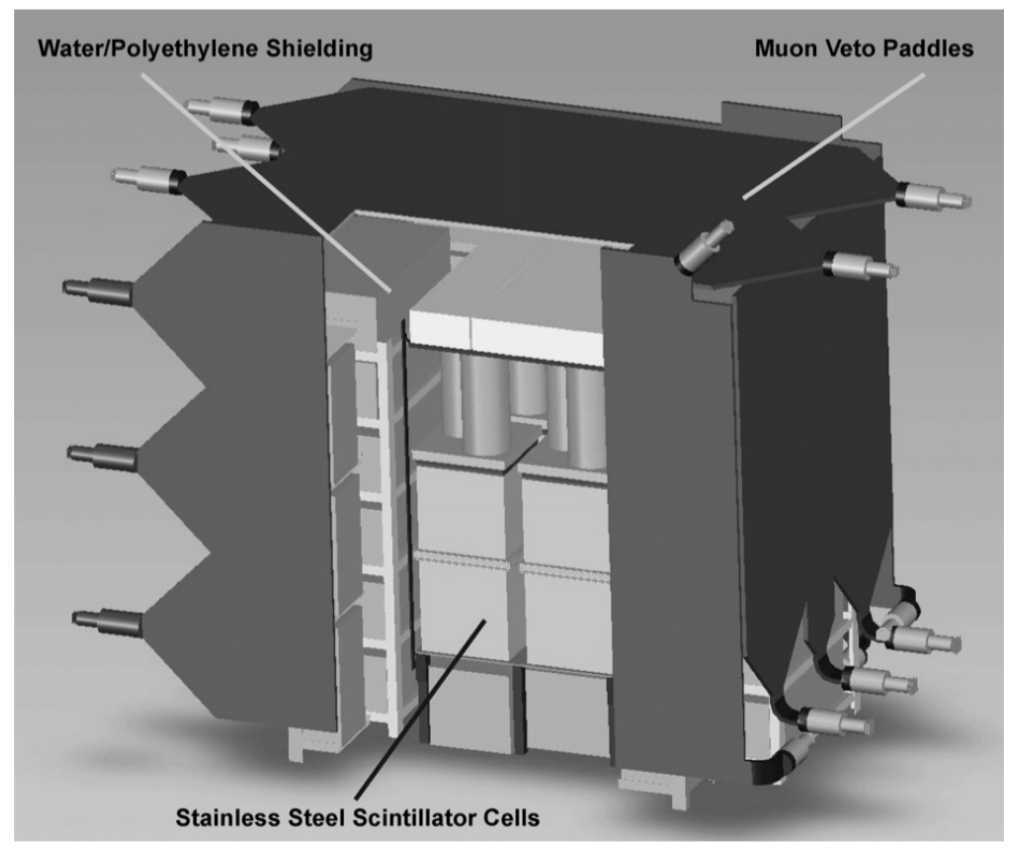
\includegraphics[width=0.5\linewidth]{Chapter1/Figs/SongsS1Detector.jpg}
 \captionof{figure}{A cut away diagram of the SONGS1 detector, showing the major subsystems. From \cite{Bowden_2007}.} 
 \label{fig:SongsS1Detector}
\end{figure}

\begin{figure}[!h]
\centering
\begin{subfigure}{.5\textwidth}
  \centering
  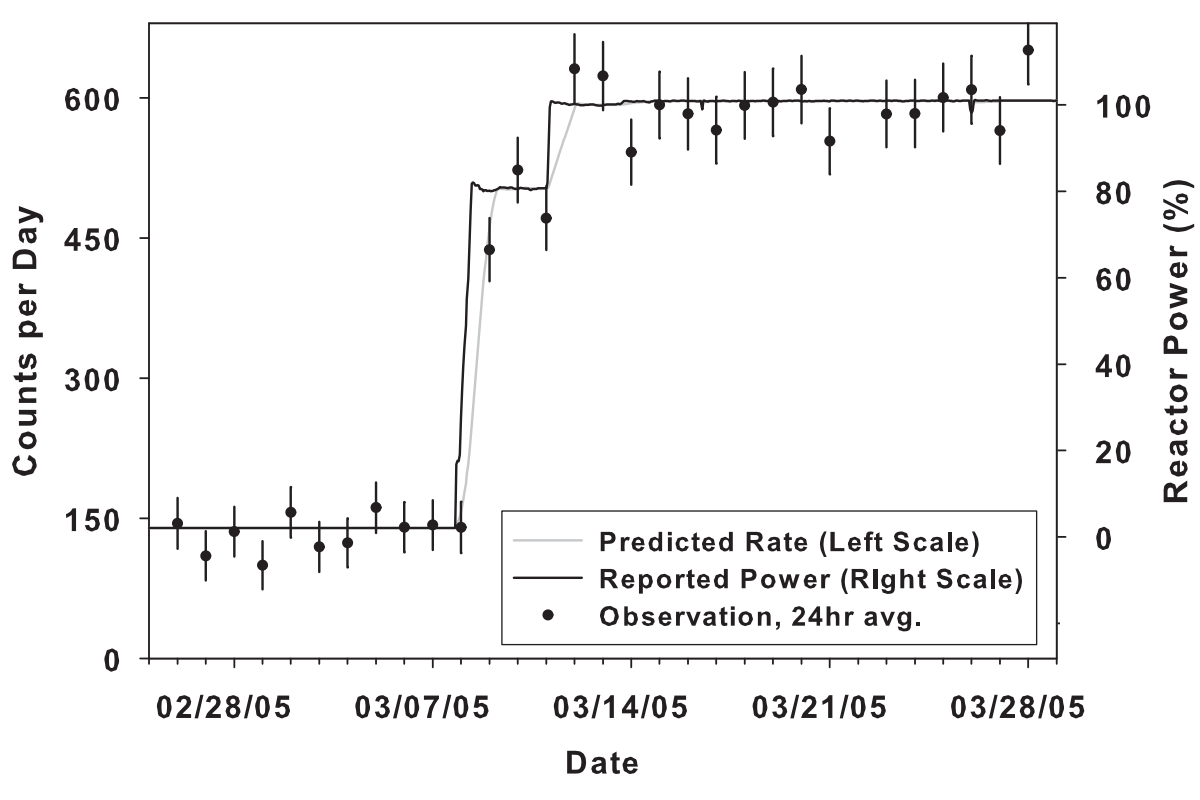
\includegraphics[width=\linewidth]{Chapter1/Figs/reactorPowerSongsS1.png}
  \captionsetup{width=.9\linewidth}
  \caption{}
  \label{subFig:reactorPowerSongsS1}
\end{subfigure}%
\begin{subfigure}{.5\textwidth}
  \centering
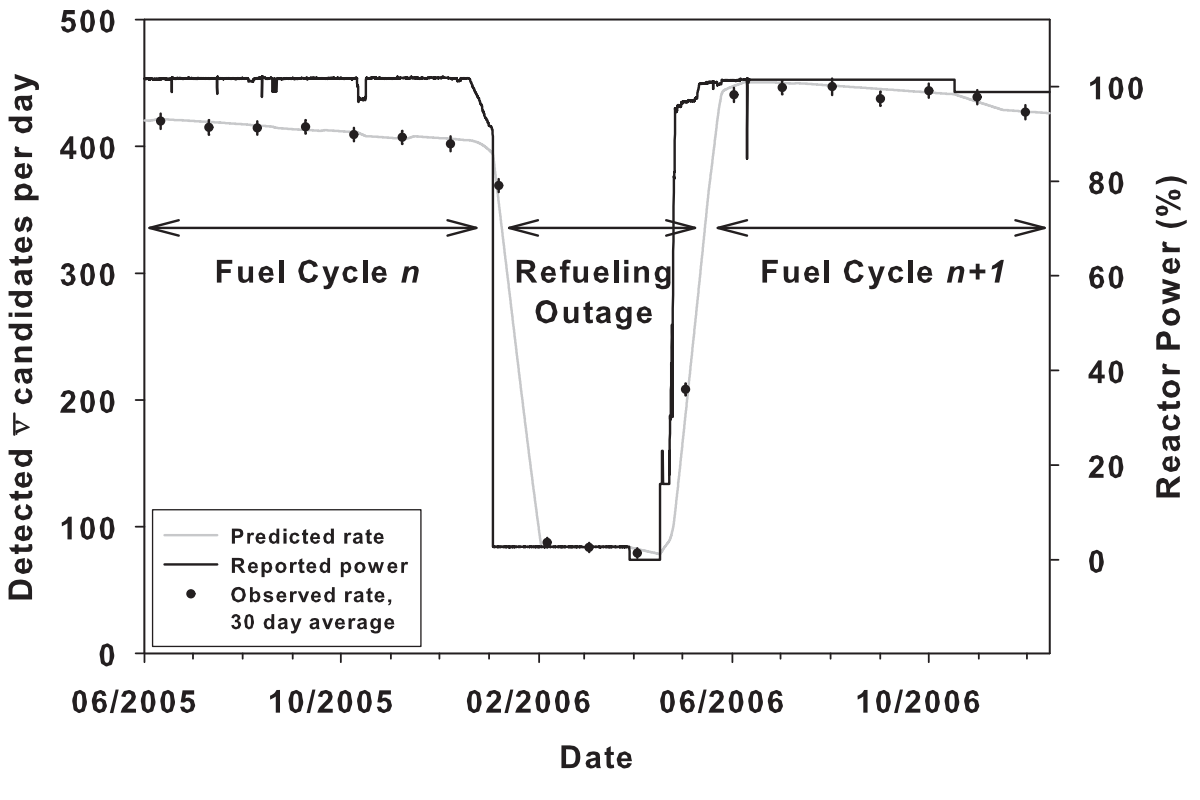
\includegraphics[width=\linewidth]{Chapter1/Figs/reactorRefulingSongs1.png}
  \captionsetup{width=.9\linewidth}
  \caption{}
  \label{subFig:reactorRefulingSongs1}
\end{subfigure}
\caption{Reactor Power and measured $\bar{\nu_e}$ from the SONGS1 core at reactor on in (a) and refuelling in (b). The measured rate approximates the power well. From \cite{Bowden_2008}.}
\label{fig:reactorPowerAndRefuelingSongsS1}
\end{figure}

\subsection{PANDA}
The Plastic Anti-Neutrino Detector Array (PANDA) \cite{PANDA_2012}, \cite{PANDA_2014}, \cite{PANDA_tgf}, \cite{IIRIE_Panda_2021}, is a segmented detector that uses plastic scintillator bars and gadolinium (Gd) embedded between the bars as shown by figure \ref{subFig:pandaClose}, with the Gd neutron interaction shown by equation \ref{equ:gadolinumNAbsorption}. The orientation of the bars can be seen in figure \ref{subFig:pandaFar} with each layer of bars parallel to each other. The bars dimensions are 10\,cm$\times$10\,cm$\times$100\,cm with two 10\,cm$\times$10\,cm$\times$10\,cm acrylic cubic light guides glued to both ends of the plastic scintillator and optical cement capped with PMTs at either end of the bars for data collection. The Gd doped sheets are inserted between the bars \cite{PANDA_2014}. The interior of a plastic scintillating bar can be seen in figure \ref{subFig:pandaClose} which also shows the prompt and delayed event of an $\bar{\nu_e}$ event. In addition, calibrations and comparison to GEANT4 \cite{Agostinelli:2002hh} have been performed with a baseline of a $^{60}$Co with reasonable agreement between the calibration source and the simulated response \cite{PANDA_2012}. 

\begin{equation}
n + {^{155,157}Gd} \rightarrow {^{156,158} Gd} + \gamma (\sim 8\,MeV)
\label{equ:gadolinumNAbsorption}
\end{equation}

\begin{figure}[!h]
\centering
\begin{subfigure}{.5\textwidth}
  \centering
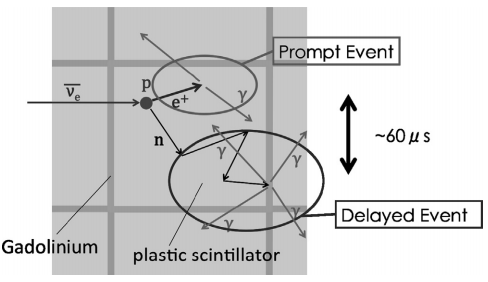
\includegraphics[width=\linewidth]{Chapter2/Figs/Raster/Panda_close.png}
  \captionsetup{width=.9\linewidth}
  \caption{}
  \label{subFig:pandaClose}
\end{subfigure}%
\begin{subfigure}{.5\textwidth}
  \centering
  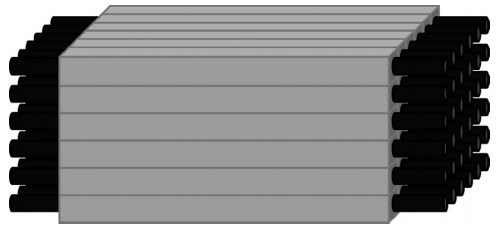
\includegraphics[width=\linewidth]{Chapter2/Figs/Raster/Panda_far.png}
  \captionsetup{width=.9\linewidth}
  \caption{}
  \label{subFig:pandaFar}
\end{subfigure}
\caption{PANDA detector interior and exterior. The interior is shown in (a) which also shows an $\bar{\nu_e}$ interaction with prompt and delayed components. The exterior of PANDA is shown in (b). The bars are clustered together with photon multiplier tubes at the end to measure photons. From \cite{PANDA_2014}.}
\label{fig:pandaCloseFar}
\end{figure}

%The bars are not positioned perpendicularly in the $z$ direction (figure \ref{subFig:pandaFar}). Therefore tracking is more difficult in PANDA, due to not having specific $x$ and $y$ coordinates, this makes vetoing cosmic $\mu$ (a major source of background) potentially harder in PANDA than if the bars were perpendicular. 
%The photon multiplier tubes (PMTs) used in PANDA are also expensive, the PANDA36 shown in figure \ref{subFig:pandaFar} is much smaller than the proposed final design of 100 channels and 1m$^3$ \cite{PANDA_2012} but PANDA is being built in stages because of the expense of these components. However, the potential for measuring many photons with high efficiency makes PMTs attractive. Both Lesser PANDA (16 channels) and PANDA36 have been deployed by van with background measurements and reactor measurements being taken from inside the van \cite{PANDA_2012}, \cite{PANDA_2014}. But due to the flammable nature of petrol and diesel, it is unclear whether reactor operators would be open to having a van stationed indefinitely outside their reactor buildings. PANDA36 has also been used for monitoring Terrestrial $\gamma$-ray Flashes (TGFs) from thunderstorms to allow for further background reduction at nuclear sites\cite{PANDA_tgf}.
Owing to the cost of PMTs, PANDA has been built in stages.  Both Lesser PANDA (16 channels) and PANDA36 have been deployed by van with background measurements and reactor measurements being taken from inside the van \cite{PANDA_2012}, \cite{PANDA_2014}. For example, PANDA36 has been used for monitoring Terrestrial $\gamma$-ray Flashes (TGFs) from thunderstorms to allow for further background reduction at nuclear sites\cite{PANDA_tgf}. In 2016 PANDA was upgraded to its final size, 100 channels. The PANDA100 detector started taking measurements at the Ohi power plant in 2018 for background subtraction and then made measurements of neutrino events in 2019 from Ohi reactors 3 and 4, at a standoff of 45\,m and 100\,m from the reactor cores \cite{Iwata_2019}. The results of the neutrino measurements from the reactors is shown in figure \ref{subFig:Panda_spectrumOfIbdCandidates} and the background spectrum is shown in \ref{subFig:Panda_SpectrumOfCosmicProducts}. The results from PANDA's deployment are very impressive with an $\bar{\nu}$ rate of 175.8 $\pm$ 34.4 day$^{-1}$ \cite{IIRIE_Panda_2021}. Of particular interest in the PANDA results is the neutrino spectrum produced in figure \ref{subFig:Panda_spectrumOfIbdCandidates} as it resembles the expected shape from Muller 2011 \cite{Mueller_2011} and by Sonzogni \cite{sonzogni_nucStrcutre_2015} (see figure \ref{fig:anSpectraIsotopes}).

\begin{figure}[!h]
\centering
\begin{subfigure}{.4\textwidth}
  \centering
  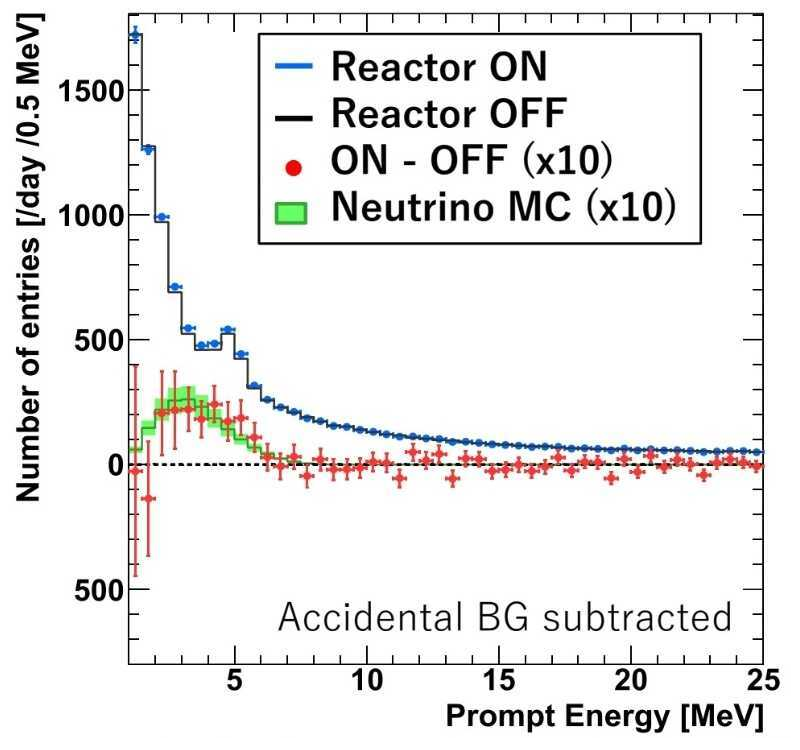
\includegraphics[width=\linewidth]{Chapter1/Figs/Panda_spectrumOfIbdCandidates.png}
  \captionsetup{width=.9\linewidth}
  \caption{}
  \label{subFig:Panda_spectrumOfIbdCandidates}
\end{subfigure}%
\begin{subfigure}{.4\textwidth}
  \centering
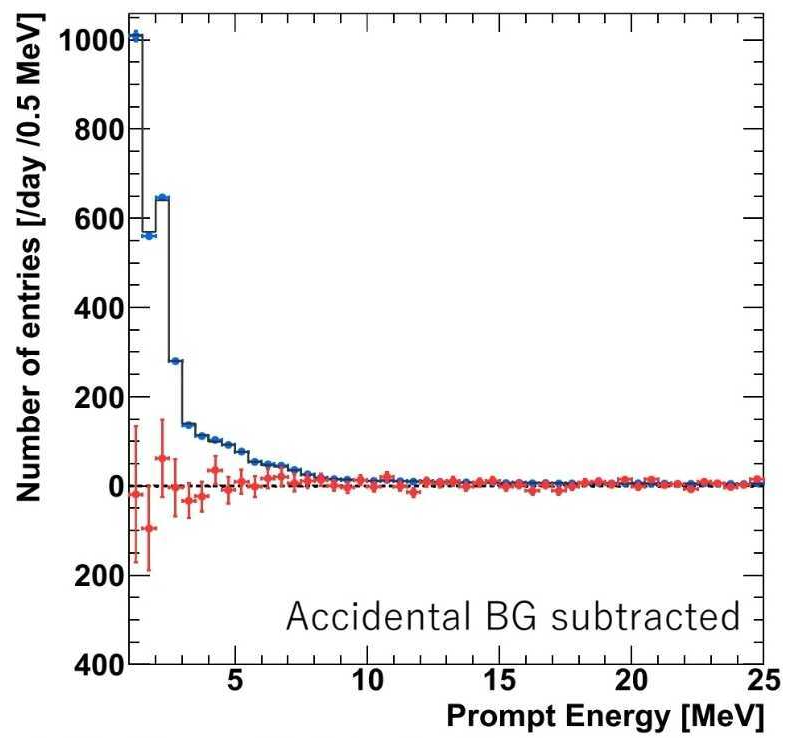
\includegraphics[width=\linewidth]{Chapter1/Figs/Panda_SpectrumOfCosmicProducts.png}
  \captionsetup{width=.9\linewidth}
  \caption{}
  \label{subFig:Panda_SpectrumOfCosmicProducts}
\end{subfigure}
\caption{Results from the PANDA deployment between 2018 -- 2019. In (a) Number of observed neutrinos is 175.8 $\pm$ 34.4 [day$^{-1}$] to within 5.10 $\sigma$. In (b) the spectrum of cosmic products is shown to go to zero once accounting for background. From \cite{IIRIE_Panda_2021}.}
\label{fig:Panda_spectrumOfIbdAndCosmicCandidates}
\end{figure}

% \subsection{SoLid and CHANDLER}
% The SoLid detector is a plastic scintillating detector that uses wavelength shifting (WLS) fibres with MPPCs at the end to read out fibre signals and adjacent 5\,cm $\times$ 5\,cm $\times$ 5\,cm cubes being lit up at similar time intervals to discern particles \cite{Solid_proposal}. There is a prompt signal outputted from the positron in the plastic cubes and a delayed signal from the $^6$LiF:ZnS(Ag) screen interacting with neutrons as shown in figure \ref{fig:SolidCubeDiagram}. The prompt positron response and delayed neutron response is similar to the other experiments mentioned. In SoLid $^6$Li is used as the neutron capture agent (equation \ref{Li_interact_eq}), which produces an $\alpha$ and a 4.78\,MeV $\gamma$ \cite{Solid_readout}. The $\gamma$ signal is ignored because the $\alpha$ signal produced is clear and produces a specific pulse shape signal \cite{Solid_readout} which has a very minimal background due to its specific pulse shape. Setting it apart from other experiments that use the 8\,MeV Gd cascade. 

% \begin{equation}
% n + {^6Li} \rightarrow {^3H} + \alpha +4.78\,MeV
% \label{Li_interact_eq}
% \end{equation}

% \begin{figure}[!h]
%  \centering
%  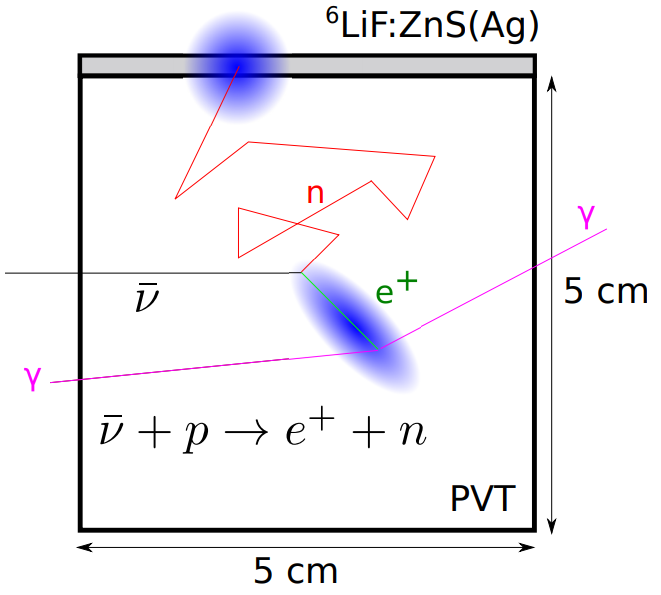
\includegraphics[height=58mm]{Chapter2/Figs/Raster/SoLid_cube.png}
%  \captionof{figure}{SoLid cube during an inverse beta decay event $\bar{\nu}$ decays into a positron and neutron via equation \ref{inverse_beta_decay}, delayed neutron is captured by $^6$LiF:ZnS(Ag) screen, positron gives the prompt response. From \cite{Solid_readout}.} 
%  \label{fig:SolidCubeDiagram}
% \end{figure}

% The challenge with using $^6$Li as a neutron capture agent is producing enough light for pulse shape discrimination (PSD) to be used in the analysis. The $\alpha$s need to be captured by the sulphur in the $^6$LiF:ZnS(Ag) screen which then emits a specific $\gamma$ into the plastic which in turn produces electrons via Compton scattering which are then captured by WLS fibres. An alternative method to this is that proposed by CHANDLER (Carbon Hydrogen $\bar{\nu}$ Detector with a Lithium Enhanced Raghavan-optical-lattice) \cite{aap2015}. Which uses PMT's and a Raghavan-optical-lattice to counter-act the low light issues in SoLid. However, the CHANDLER design also brings challenges as the detector cannot be too large otherwise attenuation and containment of events prevent signals from being read.
% \\\\The SoLid experiment has collected data up to June 2020 and is current deployed at the BR2 reactor in Belgium [6300 mm–8938 mm] from the nominal reactor core \cite{Abreu_2021}. The results from the period of July 2018 -- August 2019. The trigger strategy for for SoLid neutrinos relies solely on triggering on a scintillation signal generated in the
% neutron detection screens (NS). The values for the NS rate for SoLid at BR2 can be seen in figure \ref{fig:solidReults}. As such figure \ref{fig:solidReults} shows how the SoLid detector is triggering as expected for an $\bar{\nu}$ detector. Currently the SoLid collaboration approximates the detector is subject to $\sim$ 1000 per day though the short bursts the BR2 causes difficulty through off-equilibrium effects \cite{Abreu_2021}. 
% \begin{figure}[!h]
%  \centering
%  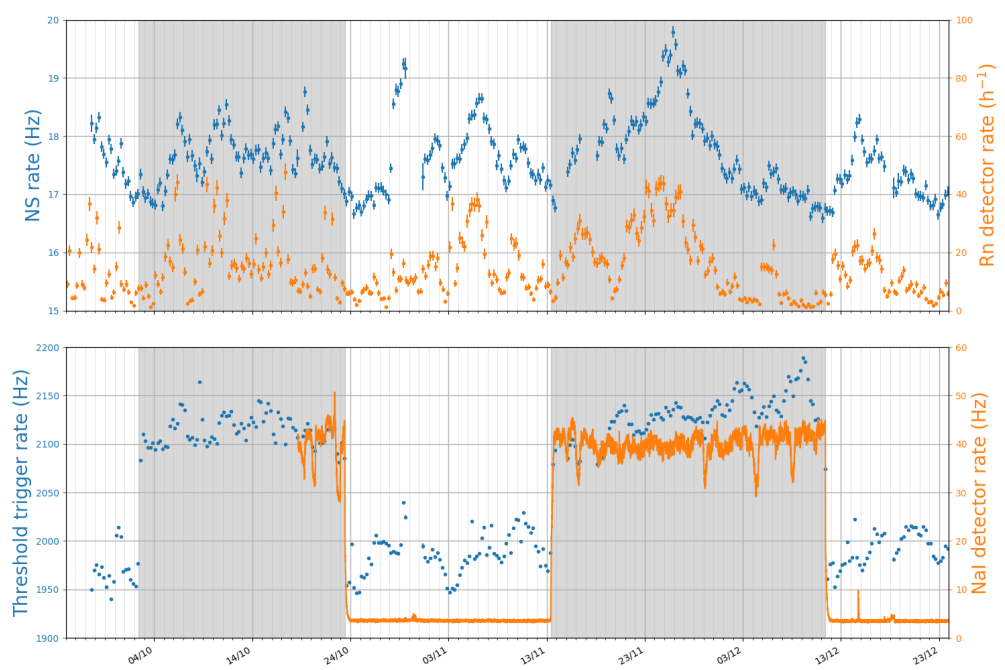
\includegraphics[width=0.7\linewidth]{Chapter1/Figs/SoLidResults.png}
%  \captionof{figure}{Results from SoLid detector at BR2. (Top) Long term trends of the NS rate after muon contamination removal (blue) and the airborne radon detector rate (orange). (Bottom) Long term trends of the threshold trigger rate (blue) and the NaI detector rate (orange). Reactor ON periods are shown as grey bands. From \cite{Abreu_2021}} 
%  \label{fig:solidReults}
% \end{figure}

\subsection{RENO} \label{subSec:reno}
%Papers found by this collaboration include \cite{reno_may_2012}, \cite{reno2013},  \cite{reno_may_2019}. 
RENO was the first long base line experiment to see $\Bar{\nu_e}$ disappearance \cite{Olive_2014}. The RENO experiment consists of two detectors at a distance of 294\,m for the near detector, and 1383\,m for the far detector \cite{reno_may_2012}. A schematic of the detectors used in RENO can be seen in figure \ref{fig:RENO_detector}, illustrating that this detection system uses Gd-doped liquid scintillator with PMTs. By measuring the prompt energy from both the near and far RENO detectors a spectrum of energies for both can be produced (figure \ref{fig:RENO_Spectrum}). There is a clear $\bar{\nu_e}$ deficit visible between the near and far detector spectra in figure \ref{fig:RENO_Spectrum} \cite{reno_may_2012}. Figure \ref{fig:RENO_Spectrum} also shows the ratio between the near and far detectors further highlighting the neutrino deficit. 

\begin{figure}[!h]
\centering
\begin{minipage}{.45\textwidth}
  \centering
  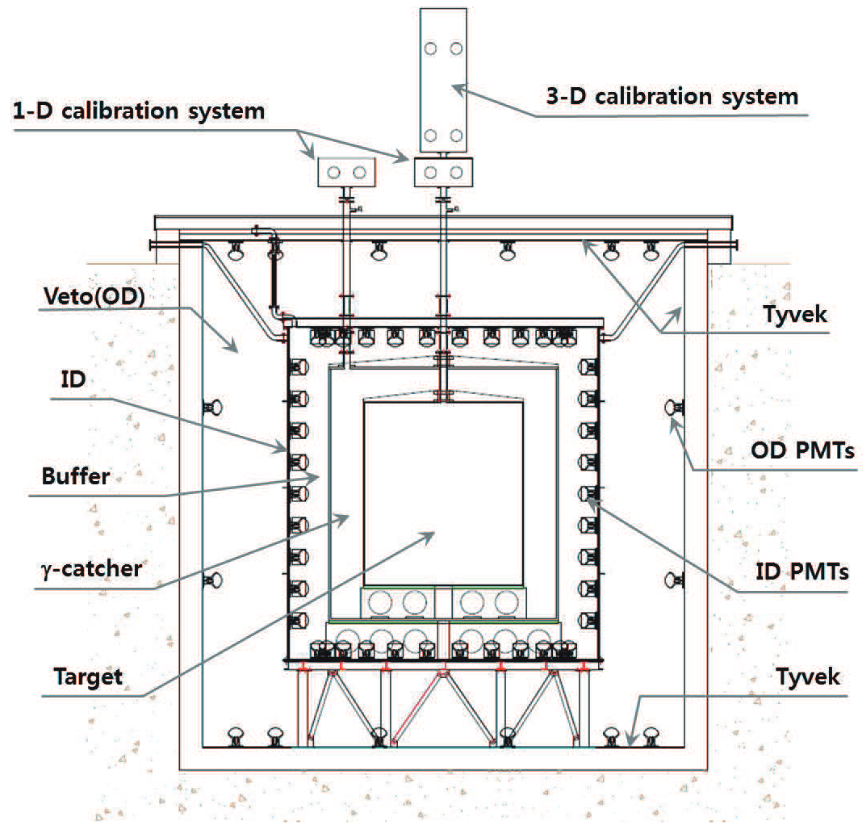
\includegraphics[width=\linewidth]{Chapter2/Figs/Raster/RENO_detector.png}
  \captionof{figure}{Schematic view of a RENO detector. The near and far detectors are identical. The detector seen in this figure consists of a main inner detector (ID) and an outer veto detector (OD). From \cite{reno_may_2012}.} 
  \label{fig:RENO_detector}
  \vspace{2.39cm} %1 line = 0.478cm % 2 lines = 0.956cm % 3 lines= 1.434cm % 4 lines = 1.912cm % 5 lines = 2.39cm
\end{minipage}%
\qquad
\begin{minipage}{.45\textwidth}
  \centering
  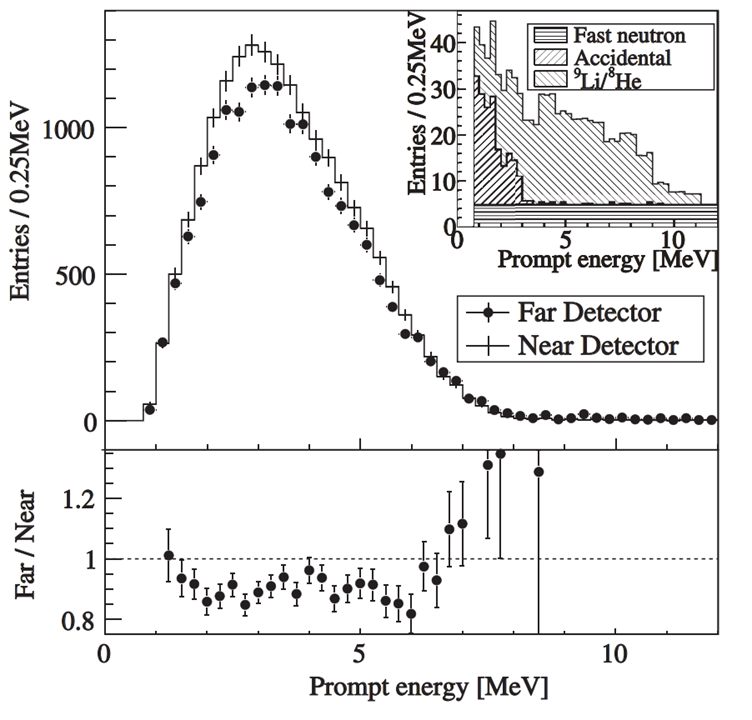
\includegraphics[width=\linewidth]{Chapter1/Figs/Raster/RENO_Spectrum.png} 
  \captionof{figure}{Observed spectrum of the prompt signals in the far RENO
detector compared with the non-oscillation predictions from the measurements in the near RENO detector. The backgrounds shown in the inset are subtracted for the far spectrum. The background fraction is 5.5\,\% (2.7\,\%) for far (near) detector. Errors are statistical uncertainties only. Bottom: The ratio of the measured spectrum of far detector to the non-oscillation prediction. From \cite{reno_may_2012}.}
  \label{fig:RENO_Spectrum}
\end{minipage}
\end{figure}

RENO's results in 2012 were consistent with neutrino oscillations to within 4.9 $\sigma$ from six 2.8\,$GW_{th}$ reactors \cite{reno_may_2012}. RENO was able to constrain the measurement of $\theta_{13}$ (a component Pontecorvo–Maki–Nakagawa–Sakata (PMNS) that will be explained in section \ref{sec:neutrinoFlavours}) in 2012 using a rate based analysis to produce  $\sin^2{2\theta_{13}}$ = 0.113$\pm0.013$(stat.)$\pm0.019$(syst.) which was consistent with the findings that Double Chooz would produce later. These results were revised once again in 2013 using 800 days of live time to $\sin^2{2\theta_{13}}$ = 0.100 $\pm$ 0.010(stat) $\pm$ 0.015 (sys.) corresponding to 6.3 $\sigma$ significance \cite{reno2013}. The focus of the RENO collaboration has since shifted to analysing the 5\,MeV reactor anomaly \cite{reno_may_2019}. 

\subsection{Double Chooz} \label{subSec:doubleChooz}
%I feel like Double Chooz, Reno, KamLAND and Daya Bay are all very similar, liquid scintillating detectors with Gd doping initlally trying to find theta_13 but then transitioned to the 5 MeV reactor bump all of these are not proliforation focussed but measrument focussed experiments 
%Double Chooz is probably one of the most well known reactor monitoring programs. \cite{abe2014improved} goes over some of the details and I have already mentioned it here. Also the \cite{lasserre2006} reference may be useful, used it once before in the first year literature survey. I've also cited \cite{Abe_2012} in the past and that may prove useful here. Further the reference \cite{Olive_2014} may also be of use. Double Chooz is a good one to cite because its clearly not in competition with VIDARR. It requires to be very close and a big hole dug underground and uses gadolinium suspended in liquid organic scintillator. Which is not cheap or portable, it does however give significantly better measurements for the disappearance of $\bar{\nu}$s which the above references mention.

%The Double Chooz experiment is an evolution of the original Chooz experiment which was set up at the Chooz nuclear power plant in France\cite{lasserre2006}. Both of these experiments attempted to measure the $\Bar{\nu_e}$ disappearance from the same reactor however the original Chooz experiment was unable to see any disappearance to a 90$\,\%$ confidence level \cite{Apollonio_2003}. Both experiments used gadolinium doped liquid scintillator with the Double Chooz experiment having a near and far detector at 280\,m and 1050\,m respectively\cite{lasserre2006}. Finally, in 2012 $\Bar{\nu_e}$ disappearance was observed at the Double Chooz experiment \cite{Abe_2012}. These results were improved further in 2014 \cite{abe2014improved}.
The Double Chooz experiment followed the Chooz experiment to measure the disappearance of $\bar{\nu_e}$s from the Chooz nuclear power plant in France \cite{lasserre2006}. With the Chooz experiment failing to measure disappearance to the 90\,\% confidence level \cite{Apollonio_2003}, the upgrade to Double Chooz replaced the detector at standoff of 1050\,m and added a near detector at 280\,m and saw disappearance in 2012 \cite{Abe_2012}. These results were further improved with data taking up to 2014 \cite{abe2014improved}.

\begin{figure}[!h]
 \centering
 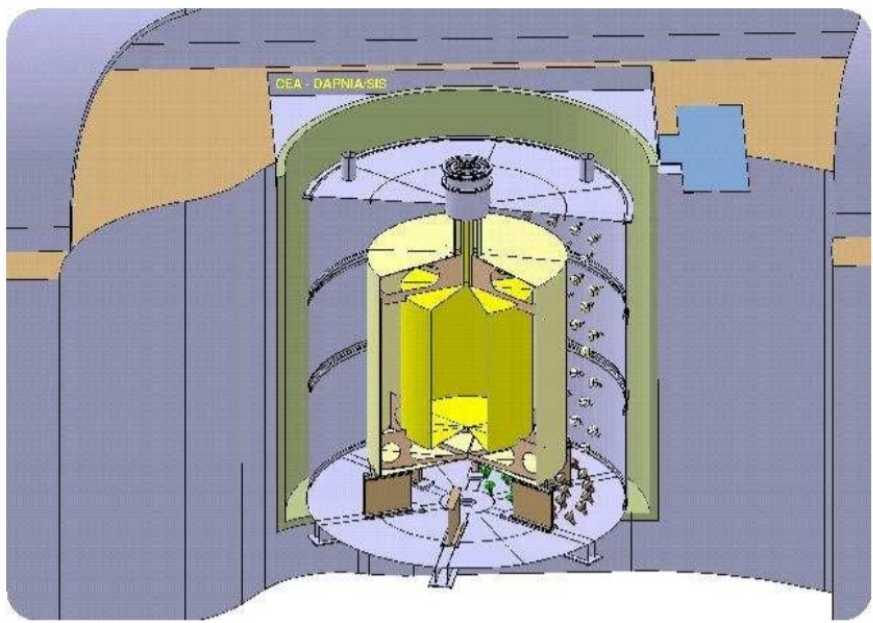
\includegraphics[width=0.5\linewidth]{Chapter1/Figs/doublChoozDetectorDiagram.jpg} %height of this plot had to be adjusted because of its unusal diemensions
 \captionof{figure}{The Double Chooz-far detector at the Chooz underground site (7\,m high and 7\,m in diameter). A total of 10.3\,m$^3$ of dodecane+PXE-based liquid scintillator doped with gadolinium is contained in a transparent acrylic cylinder surrounded by the $\gamma$ region (22.6\,m$^3$) and the buffer (114.2\,m$^3$). From \cite{lasserre2006}.} %~can be used as a kind of place holder in latex
 \label{fig:DoubleChoozFarDetector}
\end{figure}
The Double Chooz experiment uses detectors placed underground to allow for a large amount of overburden to reduce background rates. The overburden for the near detector is 30\,m resulting in 300 meter water equivalent (m.w.e) \cite{lasserre2006}. This high overburden was chosen to maximise the true-neutrino-signal to background ratio. The far detector only has 70-80\,m.w.e and so the outer shielding is different \cite{lasserre2006}. The far detector consists of a 10.3\,m$^3$ volume filled dodecane+PXE based liquid scintillator doped with gadolinium contained in a transparent acrylic cylinder to act as a target, surrounded by a 22.6\,m$^3$ volume to measure background gamma radiations. To minimise background, a 114\,m$^3$ buffer region shields the inner-detector. The near and far detectors are identical inside the PMT support structure but the outer shielding is not identical due to the difference in cosmic ray backgrounds at the near and far sites \cite{lasserre2006}. Although the Double Chooz measurement  was not the first to measure the rate of $\bar{\nu}$ disappearance \cite{reno_may_2012} like RENO, it was able to produce a spectrum of the disappearance for $\theta_{13}$ which can be seen in figure \ref{doubleChoozSpectrumNoCaption}. The measured energy spectrum (the black points in figure \ref{doubleChoozSpectrumNoCaption}), was best fitted using the parameter of $\sin^2{2\theta_{13}}$ = 0.109 $\pm$0.030(stat)$\pm$0.025(syst) which is shown as the red line in figure \ref{doubleChoozSpectrumNoCaption} \cite{Abe_2012}. The data exclude the no-oscillation hypothesis at 99.8$\%$ CL (2.9$\sigma$)\cite{Abe_2012}. This data was further expanded upon in 2014 producing a result of $\sin^2{2\theta_{13}}$ = 0.090$^{+0.032}_{-0.029}$ using 467.90 live days of data to within $3.0\sigma$ \cite{abe2014improved}.
\begin{figure}[!h]
 \centering
 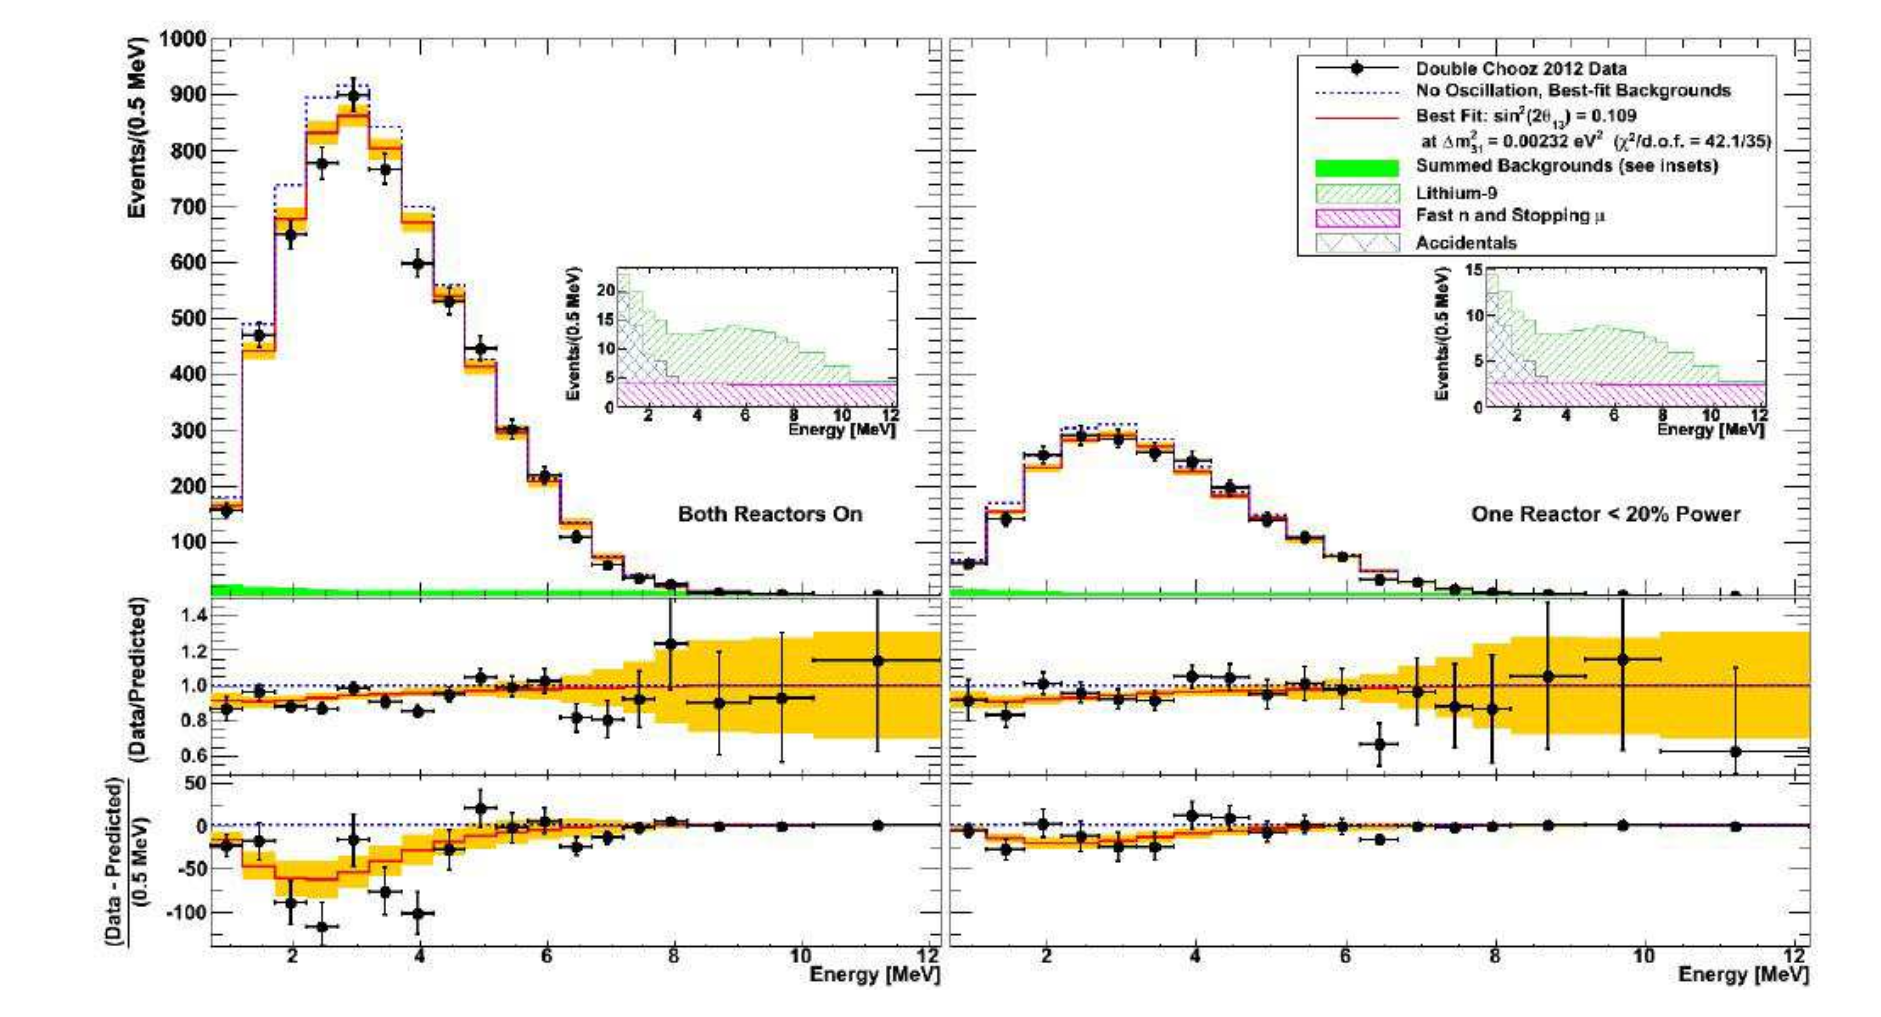
\includegraphics[width=0.8\linewidth]{Chapter2/Figs/Raster/doubleChoozSpectrumNoCaption.png} %Just use linewidth for this one
 \captionof{figure}{Double Chooz measured prompt energy spectrum for each integration period (data points) superimposed on the expected prompt energy spectrum, including backgrounds (green region), for the no-oscillation (blue dotted curve) and best-fit (red solid curve) at $\sin^2{2\theta_{13}}$ = 0.109 and $\Delta$m$^2_{31}$ = 2.32$\times$10$^{-3}$eV$^2$. Inset: stacked spectra of backgrounds. Bottom: differences between data and no-oscillation prediction (data points), and differences between best fit prediction and no-oscillation prediction (red curve).The orange band represents the systematic uncertainties on the best-fit prediction. From \cite{Abe_2012}} %~can be used as a kind of place holder in latex
 \label{doubleChoozSpectrumNoCaption}
\end{figure}

\subsection{Other Experiments}
This list of reactor experiments is not exhaustive near-field examples such as SoLiD \cite{Solid_readout}, CHANDLER \cite{aap2015}, and Nucifer \cite{nucifer2016} were not touched upon. Whilst these experiments may have interesting differences from VIDARR and RMon (both SoLid and CHANDLER use Li instead of Gd and Nucifer is a liquid detector) the utility of these experiments is very similar to the PANDA and SONGS1 examples discussed. The reason SONGS1 was focused on is because it was the first proof of concept for near-field reactor monitoring. Whilst PANDA was focused on as its technology is quite similar to VIDARR's with the near-field ranges of $\sim$ 45\,m -- 100\,m from commercial reactor cores being similar to the expected deployment ranges for VIDARR and the $\sim$ 60\,m range RMon was deployed at. 
\\\\Similarly there are more far-field experiments than Double Chooz and RENO. For example, the Daya Bay experiment in China uses similar technology to both RENO and Double Chooz to measure $\bar{\nu_e}$s from reactors \cite{DayaBay2007Precision}. The Daya Bay experiment has also started to investigate the reactor anomaly at 5\,MeV, similar to RENO \cite{Daya_Bay_2017}. Another experiment of interest is the WATCHMAN collaboration which has the goal of far-field reactor monitoring using $\bar{\nu_e}$s originally planned to be deployed in the U.S.A \cite{askins2015physics} it has since become a joint U.S -- U.K project and will be deployed at Boulby mine \cite{burns2018remote}. Its technology is in a state of flux but will use Gd in a fluid detector. There has been some external collaboration between the VIDARR experiment and the WATCHMAN experiment. In particular, the application of the DANCE calorimeter data to implement the DICEBOX package for Gd which VIDARR has also taken advantage of as part of this work. 

%Nucifer is also similar to the other experiments being a scaled-down version of Double Chooz, Daya Bay and RENO using Gd doped liquid scintillator with the goal of near field reactor monitoring \cite{nucifer2016}

% The original prototype to VIDARR deployed at the Wylfa reactor site from June 2014 - Feburary 2016 based on the T2K ND280 ECal was unofficially referred to as RMon by the collaboration. However, the experiment's name has now been finalised as the Verification Instrument for the Direct Assay of Radiation at Range or VIDARR and as such the prototype to VIDARR will be referred to as ProtoV. This naming convention is adopted from the SuperK experiment as the upgrade from Kamiokande to Super Kamiokande is similar in spirit to the upgrade from ProtoV to VIDARR and as such this retroactive naming convention will be applied.
\section{RMon And VIDARR detector for Nuclear Safeguards}
The University of Liverpool has developed a detector to demonstrate the potential usefulness of a $\bar{\nu_e}$ detector for safeguarding purposes. In the modern political climate where nuclear power is seen as a stable form of low carbon power generation, more nations are considering nuclear power once again. Hence the concern of atomic weapons proliferation has increased. Current safeguards for non-proliferation are dependent on accurate bookkeeping and estimations from power generation. Whilst these methods are effective, more direct methods of measuring the flux from reactors, and thereby the production of weapons-grade material, would greatly aid international institutions and watchdogs.
\\\\Between 2014 -- 2016 a prototype detector (RMon) based on the T2K ND 280 ECal \cite{Allan_2013} was deployed at the Wylfa reactor site. This deployment proved successful in measuring the reactor turn-on after a period of refuelling in 2014. However, there are improvements to the target mass, time resolution, Multi-Pixel Photon Counters (MPPCs), and temperature control which would greatly improve these results. An upgrade that implements all of these improvements is in development albeit has experienced delays due to the COVID-19 pandemic. The Verification Instrument for the Direct Assay of Radiation at Range (VIDARR) hopes to provide measurement the $\bar{\nu_e}$ flux with sensitivity and accuracy sufficient for safeguard monitoring whilst fulfilling all the positive traits the IAEA would like to see in a mobile detector \cite{IAEA_2008}.
\\\\In this thesis, the expected performance of the VIDARR detector has been characterised through GEANT4 \cite{Agostinelli:2002hh} simulations to illustrate the potential of the detector. Owing to the high degree of segmentation of the detector compared to other $\bar{\nu_e}$ reactor monitors the tracking of particles especially cosmic $\mu$ through the detector is more accurate. The data taken by the RMon detector at Wylfa has been revisited to demonstrate the detectors capability at cosmic $\mu$ tomography.

% The aim of the Verification Instrument for the Direct Assay of Radiation at Range (VIDARR) project is to demonstrate the potential usefulness of an electron $\bar{\nu}$ ($\bar{\nu_e}$) detector for safeguarding purposes. Between 2014 -- 2016 a prototype detector (RMon) based on the T2K ND 280 ECal \cite{Allan_2013} was deployed at the Wylfa reactor site. This deployment proved successful in measuring the reactor on period in 2014. However, there are improvements to the target mass, time resolution, improved Multi-Pixel Photon Counters (MPPCs), and temperature control which would greatly improve these results. An upgrade that implements all of these improvements is planned and has been characterised through GEANT4 \cite{Agostinelli:2002hh} simulations. In the modern political climate where nuclear power is seen as a stable form of low carbon power generation, more nations are considering the nuclear power once again. As such the concern of atomic weapons proliferation has increased. Current safeguards for non-proliferation are dependent on accurate bookkeeping and estimations from power generation. Whilst these methods are effective, more direct methods of measuring the flux from reactors, and thereby the production of weapons-grade material, would greatly aid international institutions and watchdogs.
% \\\\$\bar{\nu}$ reactor monitoring also has potential benefits for utilising fuel more effectively. Increasing power generation whilst decreasing the amount of nuclear waste to be stored. This potential is not yet fully realised due to the increased complexity of this method as it requires differentiating between different isotopes rather than just measuring reactor $\bar{\nu_e}$ flux. Whether this is feasible will be tested once the upgrades to VIDARR are completed and it is deployed at a new reactor site.  